\documentclass[a4paper,14pt]{extarticle}
\usepackage{cmap}				% To be able to copy-paste russian text from pdf			
\usepackage[utf8]{inputenc}
\usepackage[T1]{fontenc}
\usepackage[margin=1in]{geometry}
\usepackage[english, russian]{babel}

\usepackage[hyphens]{url}
\urlstyle{same}
\usepackage{hyperref}

\usepackage{multirow}
\usepackage{graphicx}
\usepackage{caption}
\usepackage{amsmath}
\usepackage{mathtools}

\usepackage{tikz}
\usepackage{pgfplots}
\usepgfplotslibrary{groupplots,colorbrewer,dateplot,statistics}

%\def\ishtml{1}
\ifdefined\ishtml
  % HTML mode
  \newcommand{\urlnote}[2]{\href{#2}{#1}} % Make cool link 
  \newcommand{\smallsep}{thinspace} % to be replaced with unicode 8239 later
\else
  % PDF mode
   \usepackage{libertine}
   \usepackage{libertinust1math}
   \newcommand{\urlnote}[2]{#1\endnote{\url{#2}}}  % Put URLs to endnotes
   \newcommand{\smallsep}{\kern 0.1em}
\fi

% Move footnotes to end of document
\usepackage[backref=true]{enotez}
\DeclareTranslation{russian}{enotez-title}{Примечания}

\usepackage[
	output-decimal-marker={,},
	group-separator={\smallsep},
	group-minimum-digits=3
]{siunitx}

% Shoot me if I know a better way to make decimal groups of two
\newcommand{\rateone}[1]{\num{#1}}
\newcommand{\ratetwo}[2]{\num{#1}\smallsep#2}
\newcommand{\ratethree}[3]{\num{#1}\smallsep#2\smallsep#3}

\newcommand{\ru}[1]{\begin{otherlanguage}{russian}#1\end{otherlanguage}}
\newcommand{\en}[1]{\begin{otherlanguage}{english}#1\end{otherlanguage}}
\newcommand{\ruen}[2]{#1 (\en{#2})}

\usepackage[style=alphabetic, backend=biber]{biblatex}
\addbibresource{index.bib}
\renewcommand*{\bibfont}{\small}
\setcounter{biburllcpenalty}{9000}
\setcounter{biburlucpenalty}{9500}

\author{Артём Бакулин}
\date{\today}
\title{Современный валютный рынок}

\begin{document}

\maketitle
\thispagestyle{empty}

\begin{figure}[h]
\centering
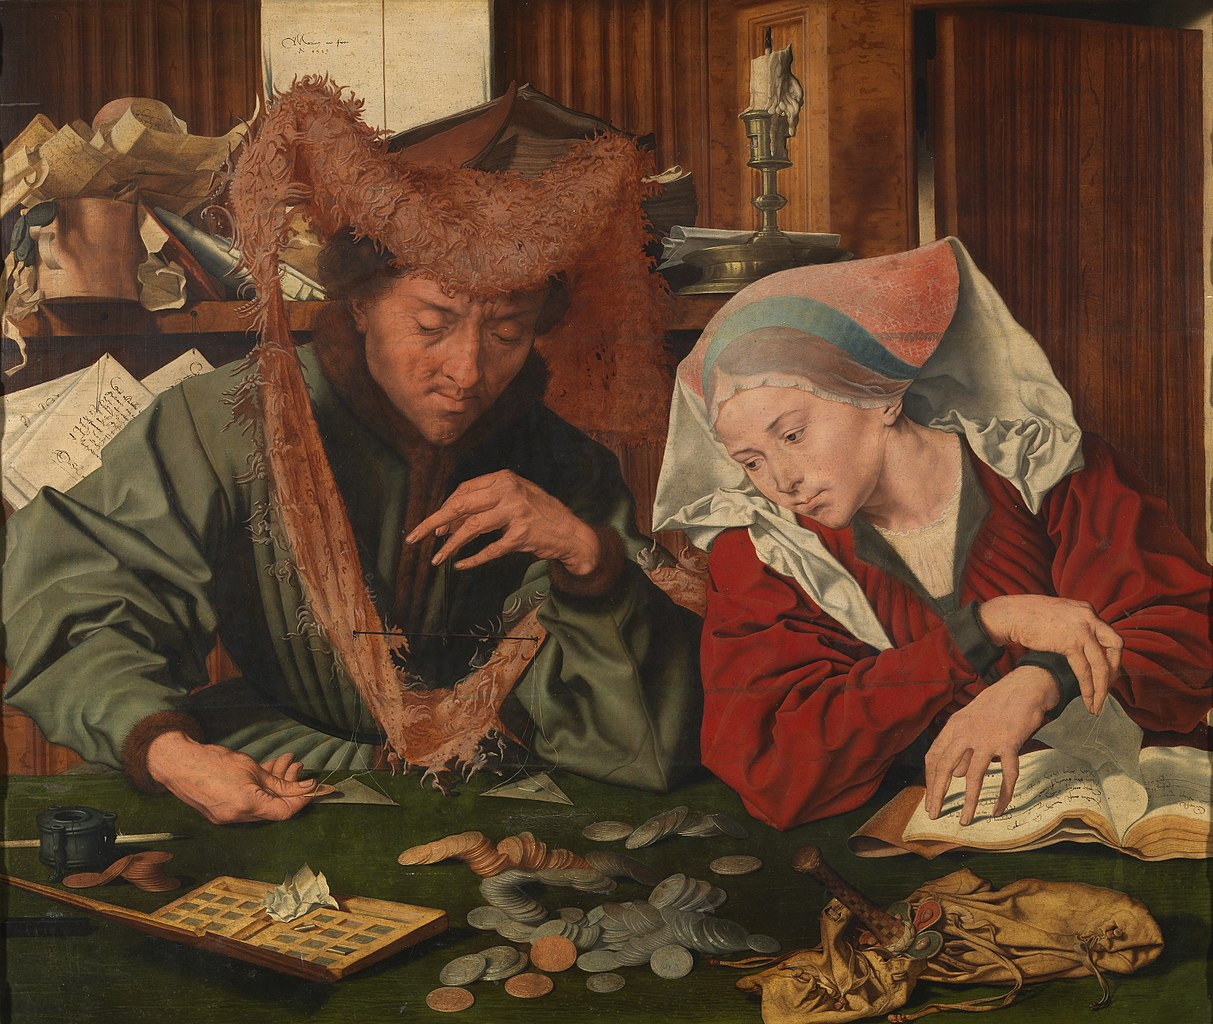
\includegraphics[width=\textwidth]{moneychanger_and_his_wife.jpg}
\captionsetup{labelformat=empty}
\caption{\small{
Маринус ван Реймерсвале. \urlnote{Меняла и его жена}
{https://commons.wikimedia.org/wiki/File:Marinus_Claesz._van_Reymerswaele_001.jpg}.
1539 г. Музей Прадо, Мадрид.
}}
\end{figure}
\newpage

\section*{Введение}

Я начал работать в Deutsche Bank программистом на Java в 2009-м году
(последствия кризиса, чудо на Гудзоне, <<Миллионер из трущоб>>, свиной грипп,
поражение сборной в Мариборе). На собеседовании мне сообщили, что я буду
работать в проекте AutobahnFX.

FX? Foreign eXchange? Мои знания о валютном рынке не отличались от знаний
среднестатистического обывателя. На углу возле дома есть обменник, но от разницы
курсов покупки и продажи дёргается глаз. В вагонах метро висит реклама
форекс-контор <<Чувствуешь разницу? На этом можно заработать!>> Газеты описывают
инвестиционные банки то как всезнающих спекулянтов, предсказывающих курсы валют
на годы вперёд, то как сборище бездарных рвачей, обрушивших мировую экономику.
<<Ну ладно, --- подумал я, --- разберёмся в процессе>>.

Эта статья --- часть того, что я выяснил, работая то над одной системой, то над
другой. Почему вам стоит прочитать её? Во-первых, это интересно. Современный
валютный рынок --- сложная распределённая система из множества независимых
акторов. Во-вторых, если вы работаете в финансах, вы можете увидеть сходство и с
другими рынками, от рынка облигаций до рынка деривативов на погоду. Наконец,
в-третьих, если в следующий кризис опять грохнется какой-нибудь инвестиционный
банк, вам будет проще читать разбор полётов в прессе.

Наш план такой. В этой статье я расскажу, как устроен валютный рынок, какова
роль крупных инвестиционных банков, какие услуги они оказывают клиентам, чем
рискуют и как зарабатывают. Во второй статье мы обсудим, может ли
рынок работать по-другому и что может случиться, если запретить банкам
заниматься этим бизнесом. Вы можете перейти сразу ко второй статье, если вам
знакомы термины <<маркет-мейкер>>, <<книга заявок>>, <<рыночный риск>> и
<<внебиржевой рынок>>.

\section*{Клиенты и маркет-мейкеры}

Начнём рассказ о валютном рынке с немецкой компании <<Рога унд копыта АГ>>,
которая продала в США партию рогов и теперь желает конвертировать часть
долларовой выручки в евро. Нет ничего проще: достаточно обратиться в банк,
клиентом которого является компания. Если казначей <<Рогов>> воспользуется
телефоном, что не редкость даже в \RN{21} веке, то между ним и сотрудником банка
состоится такой диалог:

 --- Добрый день, <<Рога>> беспокоят. Евро-доллар, 10, пожалуйста.

 --- Гутен таг. 56--58 наша цена.

 --- Купили. Данке шон.

Что только что произошло? Сначала клиент сообщил, что его интересует сделка
размером 10 миллионов евро в валютной паре евро-доллар. Размер сделки принято
указывать в первой валюте пары, а слово <<миллион>> обычно подразумевается,
потому что серьёзный бизнес меньшими суммами не торгует. Обратите внимание, что
клиент не предупредил, собирается ли он купить или продать евро.

Банк отвечает \ruen{двухсторонней}{two-way} котировкой: он готов купить у
клиента евро по 56 и продать клиенту евро по 58. Числа 56 и 58 применительно к
обмену евро на доллары выглядят непривычно, потому что мы все знаем, что курс
евро к доллару скорее близок к единичке, чем к полтиннику. Ну так это и не весь
обменный курс, а только его часть. Если сегодня с утра курс евро-доллар
составляет \rateone{1.09} плюс-минус лапоть, то нет смысла в каждом разговоре
ломать язык, называя \ruen{фигуры}{big figures} \rateone{1.09}. Все
профессионалы и так в теме. Достаточно сказать третью и четвёртую цифры после
запятой, которые называются \ruen{пипами\endnote{Очутившись как-то раз на
московском деске Deutsche, я услышал прекрасный термин <<пипки>>.}}{pips}. Таким
образом, котировка 56--58 означает готовность банка купить евро по курсу
\ratetwo{1.09}{56} и продать евро по курсу \ratetwo{1.09}{58}.

Наконец, клиент сообщает своё решение: он покупает у банка 10 миллионов евро по
курсу \ratetwo{1.09}{58}, то есть платит банку \num{10 958 000} долларов и
получает взамен \num{10 000 000} евро. Теоретически, клиент мог бы сказать
<<продаю>> и заключить обратную сделку: заплатить банку \num{10 000 000} евро и
получить \num{10 956 000} долларов. Можно и вовсе отказаться от сделки,
пробубнить <<совсем буржуи обнаглели>> и бросить трубку.

Возможно, вам бросилось в глаза, что ни клиент, ни банк не упомянули дату
расчётов. Как правило, продавец и покупатель фиксируют курс сегодня, а движение
денег по счетам происходит на второй рабочий день. Эта дата расчётов <<по
умолчанию>> называется \ruen{спот-дата}{spot date} или просто спот\endnote{Есть
несколько исключений, включая пару доллар-рубль, когда спот-дата приходится на
следующий рабочий день. Подробности на
\url{https://en.wikipedia.org/wiki/Foreign_exchange_date_conventions}.}.
Соответственно, сделка с расчётами в спот-дату называется спот-сделкой. В
принципе, клиент может попросить рассчитаться в любой другой удобный ему день,
но это будет уже не спот-сделка, а \ruen{форвард}{forward}, о котором мы
поговорим в другой раз.

Ещё немного терминологии. Курс \ratetwo{1.09}{56}, по которому банк покупает
евро, называется \ruen{бид}{bid}. Курс продажи \ratetwo{1.09}{58} называется
\ruen{аск}{ask} или \ruen{оффер}{offer}. Разность между ними, \ratetwo{0.00}{02}
или 2 пипа, называется \ruen{спред}{spread}. Среднее арифметическое курсов
покупки и продажи, \ratetwo{1.09}{57}, называется \ruen{мид}{mid} или
\ruen{мид-курс}{mid rate}.

Финансовая компания, которая даёт своим клиентам двухсторонние котировки на
валюту или другой актив, называется \ruen{маркет-мейкер}{market maker}, потому
что она, буквально, \ruen{делает}{make} цены. Ещё два термина, которые
встречаются в литературе и в этом контексте являются синонимами маркет-мейкера
--- \ruen{дилер}{dealer} и \ruen{поставщик ликвидности}{liquidity provider}.
Маркет-мейкер --- это не обязательно банк, хотя 8 из 10 крупнейших
маркет-мейкеров на валютном рынке это и правда международные инвестиционные
банки. Тройка лидеров, на которую приходится четверть рынка --- JPMorgan,
Deutsche и Citi \cite{euromoney2019}.

Прибыль маркет-мейкера --- разность между курсами покупки и продажи. Нетрудно
посчитать, что если банк продал клиенту 10 миллионов евро по 58, а затем купил у
другого клиента евро по 56, то за счёт разницы курсов он заработал $\num{10 000
000} \cdot (\ratetwo{1.09}{58} - \ratetwo{1.09}{56}) = \num{2000}$ долларов.

У меня иногда спрашивают, может ли банк продать евро, которых у него сейчас нет.
Можно ли, как мечтали герои <<Простоквашино>>, сначала продать что-нибудь
ненужное и только потом купить что-нибудь ненужное? Да, с оговорками и в
известных пределах, можно. Как мы уже знаем, обычно расчёты по валютным сделкам
происходят на второй рабочий день, а не сразу. Поэтому банк может начать с
нулевого баланса, продать клиенту евро, которых у него нет, а потом купить евро
у другого клиента.

Пока выглядит не очень сложно, не так ли? Мы все видели табло обменников с
курсами евро и доллара столько раз, что любой случайный человек с улицы с
лёгкостью объяснит, по какому курсу можно купить доллары, а по какому продать.
Если банк, по существу, работает как большой обменник, то что в этом сложного?
Покупать дешевле, продавать дороже, зарабатывать спред --- с этим справится и
пятилетний ребёнок. На некотором уровне абстракции это правда, но есть нюанс.

\section*{Управление рыночным риском}

Что может пойти не так в простой и изящной стратегии маркет-мейкера? Ответ
банален: непредвиденное движение рынка может не только оставить его без прибыли,
но и вогнать в убыток. Возможность потерять деньги из-за изменения рыночных цен
называется \ruen{рыночным риском}{market risk}.

Представьте, что вы маркет-мейкер. Вы продали <<Рогам унд копытам АГ>> 10
миллионов евро по курсу \ratetwo{1.09}{58} и теперь ждёте, когда следующий
клиент продаст вам евро по 56. Но этот второй клиент ушёл на обеденный перерыв,
поэтому вы, как говорят трейдеры, сидите <<в позиции>>. Внезапно в лентах
новостей пришло сообщение: Европейский центральный банк (ЕЦБ) сворачивает
программу количественного смягчения. Пока вы пытаетесь сообразить, что это
такое, рынок уже отреагировал: другие банки называют своим клиентам котировки
86--88, на целых 30 пипов выше, чем раньше. Вернувшись с обеда, второй клиент ни
за что не продаст вам евро по 56. Вам придётся предложить ему цену хотя бы 86,
чтобы он не ушёл к конкурентам. Каков итог? Вы купили 10 миллионов по 86 и
продали по 58. Поздравляем, вы только что потеряли \num{28 000} долларов.
Постарайтесь больше так не делать.

Как маркет-мейкер может защитить себя от потерь? Первое и самое очевидное
решение --- расширить спред между курсами покупки и продажи. Если бы вы
предложили <<Рогам>> спред не 2 пипа (56--58), а 62 пипа (26--88), то даже
движение рыночного курса на 30 пипов позволило бы вам заработать \num{1000}
долларов, продав по 88 и купив по 87. К сожалению для маркет-мейкеров, клиенты
не очень любят широкие спреды и с радостью уйдут к конкурентам, если их условия
лучше.

Второй вариант --- сделать свою цену более привлекательной для продающих
клиентов. Если вы только что продали по 58, то вы вполне можете предложить
следующему клиенту котировку \num{56.5}--\num{58.5}, даже если рыночный мид-курс
по-прежнему \num{57}. Такая котировка называется \ruen{скошенной}{skewed}. В чём
смысл? Цена покупки \num{56.5} стала выгоднее, и если клиент параллельно
общается ещё с парой маркет-мейкеров, то он с большей вероятностью продаст евро
именно вам. Вы избавитесь от риска и заработаете \num{1500} долларов. Это
меньше, чем \num{2000} долларов полного спреда, но тоже неплохо. С другой
стороны, цена продажи \num{58.5} стала хуже, и этим вы хотите отпугнуть клиента,
чтобы он ни в коем случае не покупал у вас евро, увеличивая ваш риск.

Наконец, третий путь --- <<закрыть>> позицию на межбанковском рынке. Банки
делают цены не только для клиентов, но и друг для друга. Можно позвонить другому
маркет-мейкеру, получить от него котировку с более узким спредом, скажем
\num{56.0}--\num{57.5}, и купить нужные вам 10 миллионов евро по \num{57.5}. Так
вы зафиксируете прибыль \num{500} долларов.

Внимательный читатель заметит, что котировка \num{56.0}--\num{57.5} была скошена
влево относительно мид-курса 57. Судя по всему, второй маркет-мейкер недавно
купил у своего клиента евро и теперь применяет стратегию номер 2, то есть
пытается всеми силами подстегнуть вас к сделке, которая поможет ему выйти из
позиции. Так два маркет-мейкера могут заключить сделку, которая позволит обоим
зафиксировать прибыль.

Комбинируя все три метода (управление спредом, стимулирование клиентов к
уменьшающим риск сделкам, закрытие позиций на рынке), маркет-мейкер может
более-менее стабильно зарабатывать свою копеечку при приемлемом уровне риска.
Эта копеечка не является гарантированной, и каждая конкретная сделка может
обернуться убытком, но на длинной дистанции заработать всё-таки можно.
Достаточно всегда держать в голове, какова текущая позиция, на сколько её можно
увеличить, сколько будет стоить закрыться на рынке, какие клиенты скорее всего
обратятся в ближайшее время, в каком направлении они обычно торгуют, не пора ли
давать скошенные цены, какой спред будет оправдан при текущей волатильности
рынка, не ожидается ли в течение 15 минут пресс-конференция главы ЕЦБ, есть ли
корреляция между позициями в парах евро-доллар и евро-фунт и ещё несколько
подобных мелочей.

Если вы задумались, нельзя ли переложить хотя бы часть этой работы на компьютер,
то вы мыслите в правильном направлении.

\section*{Межбанковский рынок}

Давайте посмотрим, как компьютеры помогают банкам торговать друг с другом, когда
им нужно закрыть позицию на рынке. Две самые крупные платформы,
автоматизировавшие межбанковскую торговлю --- \urlnote{Electronic Brokerage
Services
(EBS)}{https://www.cmegroup.com/trading/market-tech-and-data-services/ebs.html}
и \urlnote{Reuters
Matching}{https://www.refinitiv.com/en/products/spot-matching-forwards-matching}.
Обе платформы работают по схожим принципам, и их доли рынка приблизительно равны
\cite{golov2019fx}. Исторически сложилось, что какие-то валютные пары больше
торгуются на EBS, а другие в Reuters. Дальше я буду рассказывать про EBS, потому
что б\'{о}льшая часть сделок евро-доллар происходит именно там.

Все сделки на платформе EBS проходят через \ruen{книгу заявок}{central limit
order book, CLOB} или, как говорят русскоязычные трейдеры, через <<стакан>>.
Любая компания может с помощью приложения или API отправить свою \ruen{лимитную
заявку}{limit order}. Для этого нужно указать три параметра: направление сделки
(покупка или продажа), размер и желаемый курс. Например, <<куплю 1 миллион по
\ratethree{1.09}{56}{5} или дешевле>> или <<продам 1 миллион по
\ratethree{1.09}{57}{5} или дороже>>. Также в любой момент можно отменить заявку
или изменить размер и курс.

Сервер EBS собирает заявки, упорядочивает их по желаемой цене (заявки на покупку
--- по убыванию, заявки на продажу --- по возрастанию) и рассылает всем
участникам торгов сводку, как в таблице \ref{clob_table}.

\begin{table}[h]
\centering
\begin{tabular}{l|l|l|l|l}
\multirow{2}{*}{Уровень} & \multicolumn{2}{c|}{Покупка} &
\multicolumn{2}{c}{Продажа} \\ \cline{2-5}
& Цена & Размер & Цена & Размер \\ \hline
1 & \ratethree{1.09}{56}{5} & 1 млн. & \ratethree{1.09}{57}{5} & 2 млн. \\
2 & \ratethree{1.09}{56}{4} & 2 млн. & \ratethree{1.09}{57}{6} & 3 млн. \\
3 & \ratethree{1.09}{56}{3} & 7 млн. & \ratethree{1.09}{57}{7} & 6 млн. \\
4 & \ratethree{1.09}{56}{2} & 8 млн. & \ratethree{1.09}{57}{8} & 7 млн. \\
5 & \ratethree{1.09}{56}{1} & 9 млн. & \ratethree{1.09}{57}{9} & 6 млн.
\end{tabular}
\caption{Книга заявок на валютную пару евро-доллар}
\label{clob_table}
\end{table}

Отметим, что книга заявок анонимна. Никто кроме EBS и самого отправителя заявки
не знает, кто тот таинственный незнакомец, готовый продать 2 миллиона евро по
\ratethree{1.09}{57}{5}. Нельзя даже установить, видим мы одну заявку на 2
миллиона или две заявки по миллиону от двух разных участников рынка.

Лучшая заявка на покупку по цене \num{56.5} и лучшая заявка на продажу по цене
\num{57.5} образуют рыночный спред (его ещё называют best bid/offer, BBO). В
отличие от двухсторонней котировки маркет-мейкера, эти две цены могут исходить
от двух разных контрагентов, но это не принципиально. Для нас это выглядит так,
как если бы кто-то дал нам котировку \num{56.5}--\num{57.5} со спредом в 1 пип.

Например, чтобы продать 1 миллион евро, мы можем отправить заявку <<продам 1
миллион по \ratethree{1.09}{56}{5} или дороже>>. Система вычислит, что нашу
новую заявку можно свести (match) с уже имеющейся заявкой покупателя, и
автоматически зафиксирует сделку между нами.

За возможность заключить сделку здесь и сейчас мы дадим покупателю скидку:
продадим евро по \num{56.5}, когда мид-курс равен \num{57.0}, то есть чуть
дешевле. При размере сделки 1 миллион это будет стоить нам $\num{1 000 000}\cdot
(\ratethree{1.09}{56}{5} - \ratethree{1.09}{57}{0}) = -50$ долларов. На жаргоне
трейдеров это называется \ruen{пересечь спред}{cross the spread} или
\ruen{заплатить спред}{pay the spread}. Строго говоря, мы заплатим только
половинку полного спреда \num{56.5}--\num{57.5}, но чаще говорят именно
<<заплатить спред>>.

Вернёмся к примеру с закрытием позиции, когда мы хотели купить 10 миллионов
евро. Мы не сможем заключить столь же выгодную сделку с узким спредом в 1 пип,
потому что купить по \num{57,5} можно только 2 миллиона, а не 10. Остальные 8
миллионов обойдутся нам дороже. Отправим в EBS заявку <<куплю 10 миллионов по
\ratethree{1.09}{58}{0} или дешевле>>. Так как несколько компаний уже выразили
готовность продавать по такому курсу, EBS начнёт сводить нашу заявку с ними,
двигаясь сверху вниз по книге заявок. Так мы купим 2 миллиона по \num{57.5},
затем ещё 3 по \num{57.6} и 5 по \num{57.7}. Состояние книги заявок после
покупки нами 10 миллионов показано в таблице \ref{clob_table_2}.

\begin{table}[h]
\centering
\begin{tabular}{l|l|l|l|l}
\multirow{2}{*}{Уровень} & \multicolumn{2}{c|}{Покупка} &
\multicolumn{2}{c}{Продажа} \\ \cline{2-5}
& Цена & Размер & Цена & Размер \\ \hline
1 & \ratethree{1.09}{56}{5} & 1 млн. & \ratethree{1.09}{57}{7} & 1 млн. \\
2 & \ratethree{1.09}{56}{4} & 2 млн. & \ratethree{1.09}{57}{8} &7 млн. \\
3 & \ratethree{1.09}{56}{3} & 7 млн. & \ratethree{1.09}{57}{9} & 6 млн. \\
4 & \ratethree{1.09}{56}{2} & 8 млн. & & \\
5 & \ratethree{1.09}{56}{1} & 9 млн. & &
\end{tabular}
\caption{Книга заявок из таблицы \ref{clob_table} после исполнения заявки
<<куплю 10 миллионов по \ratethree{1.09}{58}{0} или дешевле>>}
\label{clob_table_2}
\end{table}

Интересно, что мы только что сдвинули рынок своими сделками. Изначально две
верхние заявки на покупку и продажу давали цены \num{56,5}--\num{57,5}, и
мид-курс был равен \num{57,0}. Теперь на первом уровне оказались заявки с ценами
\num{56,5}--\num{57,7}, и мид-курс стал равен \num{57,1}.

Но это ещё не всё. Сразу после сделки EBS отправит всем участникам торгов
обновлённую книгу заявок и анонимизированную информацию о недавних сделках
(<<только что прошли три сделки с курсами \ratethree{1,09}{57}{5}, \num{57.6} и \num{57.7}>>).
Сопоставив изменение книги заявок со сделками, остальные быстро вычислят, что
кому-то настолько не терпелось купить евро, что он не поскупился заплатить спред
и <<съесть>> сразу два уровня заявок на покупку. Уж не знает ли он что-то
важное? Кто-то может решить, что справедливый курс вырос, и переставить свои
заявки выше. Скажем, покупатель с заявкой на 1 миллион по \num{56,5} сдвинет её
на \num{0.2} пипа вверх до уровня \num{56.7}. Рыночный спред снова будет 1 пип
(\num{56.7}--\num{57.7}), но вокруг подросшего мид-курса \num{57.2}. Так
работает невидимая рука рынка: активный покупатель увеличивает рыночную цену.

Посчитаем, во сколько обошлась наша покупка. Средневзвешенный курс покупки
составил $(2 \cdot \num{57.5} + 3 \cdot \num{57.6} + 5 \cdot \num{57.7})/10 =
\num{57.63}$ пипа. Мы снова заплатили остальным спред, купив евро дороже
мид-курса \ratethree{1.09}{57}{0}. Это стоит $\num{10 000 000} \cdot
(\ratethree{1.09}{57}{0} - \ratethree{1.09}{57}{63}) = -630$ долларов, или по 63
доллара на каждый миллион. С другой стороны, мы же продали евро клиенту по
\num{58.0}, поэтому наша прибыль составит $\num{10 000 000} \cdot
(\ratethree{1.09}{58}{0} - \ratethree{1.09}{57}{63}) = 370$ долларов.

Можно ли как-нибудь перевернуть ситуацию и сделать так, чтобы спред платили не
мы, а другие? Без проблем. Для этого нам нужно присоединиться к ожидающим своей
очереди покупателям, вбив в систему заявку <<куплю 10 миллионов по
\ratethree{1.09}{56}{5} или дешевле>>. Получится книга заявок из таблицы
\ref{clob_table_3}.

\begin{table}[h]
\centering
\begin{tabular}{l|l|l|l|l}
\multirow{2}{*}{Уровень} & \multicolumn{2}{c|}{Покупка} &
\multicolumn{2}{c}{Продажа} \\ \cline{2-5}
& Цена & Размер & Цена & Размер \\ \hline
1 & \ratethree{1.09}{56}{5} & 11 млн. & \ratethree{1.09}{57}{5} & 2 млн. \\
2 & \ratethree{1.09}{56}{4} & 2 млн. & \ratethree{1.09}{57}{6} & 3 млн. \\
3 & \ratethree{1.09}{56}{3} & 7 млн. & \ratethree{1.09}{57}{7} & 6 млн. \\
4 & \ratethree{1.09}{56}{2} & 8 млн. & \ratethree{1.09}{57}{8} & 7 млн. \\
5 & \ratethree{1.09}{56}{1} & 9 млн. & \ratethree{1.09}{57}{9} & 6 млн.
\end{tabular}
\caption{Книга заявок из таблицы \ref{clob_table} после отправки заявки <<куплю
10 миллионов по \ratethree{1.09}{56}{5} или дешевле>>}
\label{clob_table_3}
\end{table}

Осталось немного подождать, пока на рынок не выйдет активный продавец, готовый
заплатить спред и продать евро по \num{56.5}. Когда платформа начнёт сводить
заявки, первый миллион уйдёт тому, кто раньше нас встал в очередь с заявкой по
\num{56.5}, зато все следующие миллионы достанутся нам. Если нам удастся продать
все 10 миллионов по \num{56.5}, то мы заработаем на спреде $\num{10 000 000}
\cdot (\ratethree{1.09}{57}{0} - \ratethree{1.09}{56}{5}) = 500$ долларов, или
по 50 долларов с каждого миллиона.

Недостаток пассивной стратегии <<выставить заявку и ждать>> --- полная
неопределённость времени исполнения. Продавец, готовый заключить сделку по курсу
\num{56.5}, может объявиться и через 10 миллисекунд, и через минуту, и никогда.
Напомню, что мы вышли на рынок, чтобы компенсировать риск от продажи клиенту
евро по цене \num{58.0}. Если мы будем слишком долго ждать исполнения заявки на
покупку по \num{56.5}, то запросто можем дождаться той самой пресс-конференции
ЕЦБ и скачка курса на 30 пипов. Будет крайне обидно понимать, что мы могли
избавиться от риска всего за 630 долларов, но решили сэкономить и потеряли на
порядок больше. Поэтому нужно каждый раз взвешивать экономию на спреде и риск
несвоевременного исполнения лимитных заявок.

\section*{Кредитный риск и сегментация рынка}

Компьютеризированный рынок, построенный на основе книги заявок, выглядит
многообещающе. Отправлять свои заявки могут все участники рынка, а не только
избранные маркет-мейкеры. Можно ожидать, что конкуренция продавцов снизит цены в
заявках на продажу, а конкуренция покупателей повысит цены в заявках на покупку.
В результате рыночный спред, по крайней мере для небольших сделок, будет
\'{у}же, и многим компаниям будет выгоднее совершать сделки через EBS, а не с
помощью маркет-мейкеров. К сожалению, всё не так просто.

EBS и Reuters работают по модели брокеров, то есть посредников. Когда система
EBS сводит заявки покупателя и продавца, например Deutsche и JPMorgan,
происходит двухсторонняя сделка именно между этими компаниями. Роль
компании-владельца торговой платформы похожа на работу риэлтора: помочь
покупателю и продавцу найти друг друга, взять с них небольшую комиссию за
услугу, но ни в коем случае не становиться стороной в договоре. Говоря языком
экономистов, \ruen{кредитный риск}{credit risk} ложится на продавца и
покупателя.

В чём заключается кредитный риск? Пусть, как и в примере выше, мы купили на EBS
10 миллионов по средней цене \num{57.63}. Для простоты предположим, что все 10
куплены у одного продавца. Мы ожидаем, что на второй рабочий день мы получим от
этого продавца 10 миллионов евро и сразу передадим их нашему клиенту --- <<Рогам
унд копытам АГ>>. Клиент заплатит нам \num{10 958 000} долларов, продавцу с EBS
мы заплатим \num{10 957 630} долларов. Итого, наши платежи в евро схлопнутся в
ноль, и у нас останется 370 долларов прибыли.

Если продавец с EBS разорится, то у нас будут неприятности. Нам по-прежнему
нужны 10 миллионов евро, которые придётся купить с рынка по новому рыночному
курсу. Хорошо, если рыночный курс не сильно изменился или снизился. Если же
рыночный курс сильно вырос, то нам придётся купить евро дороже
\ratetwo{1.09}{58} и зафиксировать убыток. Казалось бы, мы всё сделали
правильно, почти обеспечив себе прибыль, но неожиданный дефолт продавца оставил
нас в минусе.

Как видите, кредитный риск это не шутка. Прежде чем две компании начнут
торговать друг с другом, им придётся подписать двухстороннее соглашение, оценить
кредитоспособность друг друга, при необходимости договориться о залоге и
выставить лимиты (<<не торговать с компанией X больше, чем на миллиард>>) и
сообщить обо всём этом EBS. Система никогда не сведёт заявку продавца с заявкой
покупателя, если продавец и покупатель не проделали всю эту бюрократию. Это
имеет забавное следствие: разные клиенты EBS могут в один и тот же момент
времени видеть разное состояние книги заявок в зависимости от того, с кем из
отправителей лимитных заявок они могут торговать, а с кем нет.

Получается, что если <<Рога унд копыта АГ>> из нашего примера работают только с
Deutsche Bank, то им нет смысла подключаться к EBS. Всё равно они увидят там
только заявки того же самого Deutsche, и больше ничего. Это даже странно:
несмотря на анонимность книги заявок, конкретно <<Рога>> будут знать, как
торгует Deutsche, потому что никаких других заявок они не видят. Чтобы такого не
происходило, EBS требует, чтобы каждый новый участник имел двухсторонние
соглашения как минимум с пятью из 15-ти крупнейших дилеров \cite{cme2019elig}.

Ясно, что только довольно крупная компания или фонд может себе позволить
подключиться к EBS. Валютный рынок распадается на два сегмента: межбанковский, в
котором банки-дилеры заключают сделки друг с другом в централизованной книге
заявок, и клиентский, в котором дилеры делают двухсторонние цены для своих
клиентов.

\section*{Автоматизация клиентского рынка}

В самом начале статьи мы уже видели, как клиент может заключить сделку с банком
по телефону. До начала 00-х это был единственный способ, который требовал
вовлечения как минимум двух сотрудников банка. Это менеджер по продажам, он же
сейлз (sales), который говорит с клиентом, и трейдер (trader), который
уполномочен делать цены и управлять риском. Выслушав просьбу клиента
(<<евро-доллар, 10>>), сейлз должен был докричаться до трейдера, отвечающего за
эту валютную пару. Тот кричал в ответ <<56--58>>, сейлз кричал <<купили>> или
делал соответствующий жест, и трейдер начинал думать, что делать с риском.

Такая модель не очень хорошо масштабируется. Чтобы предложить свои услуги
большему числу клиентов, нужно нанять больше высокооплачиваемых сейлзов и
трейдеров. При этом значительную часть времени они будут отвечать на стандартные
небольшие запросы.

Лучше выдать клиенту приложение, в котором он увидит котировки на десятки
валютных пар разом, даже не пользуясь телефоном. Как только клиенту понравится
та или иная цена, он дважды кликнет мышкой, и сделка будет считаться
совершённой. Больше не нужно звонить в банк, чтобы спросить текущий рыночный
курс или купить \num{10000} евро на командировку директора. Примеры таких
приложений, которые называются \ruen{платформами одного дилера}{single-dealer
platform} --- \urlnote{Execute}{https://www.jpmorgan.com/global/markets/execute}
от JPMorgan и
\urlnote{AutobahnFX}{https://autobahn.db.com/microSite/html/fx.html} от Deutsche
Bank.

Разумеется, \ruen{ценообразование}{pricing} на этих платформах
автоматизированно, и трейдер не проводит рабочий день, вбивая двухсторонние
котировки с клавиатуры. Вместо этого он использует программу, которая собирает
данные о состоянии рынка с EBS, Reuters и из других источников и вычисляет курсы
покупки и продажи, которые можно показать конкретному клиенту. Информация о
текущей позиции тоже подаётся на вход системы ценообразования, и она может сама
решить, когда пора выдавать скошенные влево или вправо цены. Если трейдер
правильно настроит параметры системы, то она разгрузит его от рутины и позволит
сконцентрироваться на обработке нестандартных (например, слишком больших)
запросов.

Что делать клиенту, если он хочет сравнить котировки пяти маркет-мейкеров и
выбрать лучшую? Прямолинейный вариант --- установить на компьютер пять торговых
программ от пяти банков и попытаться уместить все открытые окна на большом
мониторе. Более технологичный способ --- воспользоваться услугами одного из
\ruen{агрегаторов ликвидности}{liquidity aggregator} или, по-другому,
\ruen{многодилерских платформ}{multi-dealer platform}, например
\urlnote{360T}{https://www.360t.com/} или
\urlnote{FXAll}{https://www.refinitiv.com/en/products/fxall-electronic-trading-platform}.
Эти компании вложились в техническую интеграцию со всеми крупными банками и
теперь предлагают свою собственную торговую программу, которая реализует принцип
<<одного окна>>. Не важно, хотите ли вы получить котировку от Deutsche или
JPMorgan --- вы сделаете это в одной и той же привычной программе. За это
агрегатор попросит небольшую комиссию у банка, с которым вы заключите сделку.

Уже довольно давно автоматизация достигла той стадии, когда сделки могут
заключаться без участия человека. Решение о покупке или продаже может принять
торговый алгоритм клиента. Запрос на котировку прилетает маркет-мейкеру либо
напрямую, либо через сервер агрегатора ликвидности. Курсы покупки и продажи
выдаёт система ценообразования маркет-мейкера, которая перед этим получила
информацию о состоянии рынка с серверов EBS и Reuters. Когда клиент заключит
сделку, система управления риском может сама принять решение выйти на рынок и
отправить лимитную заявку на EBS. Глобальная распределённая система работает 24
часа в сутки, с утра понедельника в Окленде до вечера пятницы в Нью-Йорке.

\section*{Внебиржевой рынок}

Подведём промежуточные итоги. Валютный рынок состоит из маркет-мейкеров, их
клиентов, а также из посредников, таких как платформы межбанковского рынка и
агрегаторы ликвидности. Обратите внимание, что на валютном рынке нет единой
торговой площадки, на которой собирались бы все желающие купить или продать
валюту. Такие рынки называются \ruen{внебиржевыми}{over-the-counter, OTC}.

Я знаю по собственному опыту, что концепция внебиржевого рынка может быть
непривычной. Для непосвящённого человека финансовый рынок это прежде всего
биржа, на которой собираются все торговцы, что-то вроде баржи из <<Незнайки на
Луне>>. Ко мне не сразу пришло осознание, что рынок вполне может работать на
основе двухсторонних договорённостей между участниками, которым совсем не
обязательно собираться всем в одном здании, или, в терминах \RN{21} века,
подключаться к единой торговой системе.

Так что валютный рынок это скорее каналы связи, соединяющие маркет-мейкеров с
клиентами и друг с другом, чем какое-то конкретное здание с колоннами в центре
города. Можете провести эксперимент: загуглите фотографии \ruen{Нью-Йоркской
фондовой биржи}{New York Stock Exchange, NYSE} или \ruen{Чикагской товарной
биржи}{Chicago Mercantile Exchange, CME}, а потом вбейте в поисковик <<Foreign
Exchange>>.

Впрочем, валютные биржи существуют, и в некоторых странах, в том числе и в
России, на них приходится значительная часть сделок. Поэтому давайте разберёмся,
как они работают.

\section*{Биржи и центральные контрагенты}

Работа биржи похожа на работу платформ межбанковского рынка, которые мы обсудили
раньше. Как правило, биржа ведёт централизованную книгу заявок, и каждый
участник торгов может отправить лимитную заявку на покупку или продажу. Пример
такого рынка у нас перед глазами --- это \urlnote{валютный рынок Московской
биржи}{https://www.moex.com/ru/markets/currency/}. Любой человек может подписать
договор с брокером, который подключит его к Московской бирже, чтобы заключать
сделки в том же <<стакане>>, что и солидные господа с миллионными заявками.

Важное отличие биржевого рынка кроется в том, что происходит после заключения
сделки. Как мы уже знаем, одной лишь книги заявок недостаточно, чтобы все
участники рынка могли торговать со всеми. Нужен механизм, который избавил бы
всех от необходимости проверять платёжеспособность каждого контрагента перед
сделкой и обеспечил бы исполнение сделок даже при банкротстве кого-то из
участников. Такой механизм есть --- это сделки с \ruen{центральным
контрагентом}{central clearing counterparty, CCP}.

В частности, я могу открыть торговый терминал и отправить на биржу заявку на
покупку \num{1000} евро за рубли по курсу, скажем, \num{73}. Когда компьютер
биржи сведёт мою заявку с заявкой на продажу от Deutsche Bank, произойдут две
сделки: между мной и биржей и между Deutsche и биржей. Биржа и станет тем
центральным контрагентом, который будет следить за исполнением сделок. Deutsche
никогда не узнает, кому он продал евро, и ему не нужно будет наводить справки о
моей благонадёжности. Если я не выполню свои обязательства, Deutsche этого не
заметит, ведь он заключил сделку с биржей, а не со мной.

Чтобы провести расчёты по сделкам даже в случае дефолта кого-то из участников,
биржа собирает со всех \ruen{гарантийное обеспечение}{margin}. Прежде чем купить
\num{1000} евро по курсу \num{73} с расчётом завтра, я должен уже сегодня внести
на счёт как минимум \num{10000} рублей. Если завтра я забуду или не смогу
перевести бирже остальные \num{63000} рублей, биржа использует моё гарантийное
обеспечение.

Завтра Deutsche передаст бирже \num{1000} евро. Биржа продаст их по новому
рыночному курсу, который может быть как выше, так и ниже вчерашних \num{73}.
Предположим, что евро подешевеет до уровня \num{71}, и тогда биржа получит
\num{71000} рублей. Биржа возьмёт из моего гарантийного обеспечения недостающие
\num{2000} и переведёт Deutsche полную сумму, то есть \num{73000} рублей. Как
видите, если курс евро не упадёт больше, чем на 10 рублей, то моего гарантийного
обеспечения хватит, чтобы биржа выполнила свою часть сделки с Deutsche и не
понесла убытков.

Таким образом, биржа может создать рынок, на котором все участники равноправны и
каждый может торговать с каждым. Книга заявок помогает покупателям и продавцам
найти друг друга, а сделки с центральным контрагентом устраняют кредитный риск.
Как ни странно, валютные биржи пока не захватили мир, и б\'{о}льшая часть сделок
по-прежнему заключается на внебиржевом рынке.

\section*{Заключение}

Валютный рынок --- это внебиржевой рынок, на котором крупные банки предлагают
клиентам двухсторонние котировки на покупку и продажу. Эти банки называются
маркет-мейкерами или дилерами. Прибыль маркет-мейкера --- разность курсов
покупки и продажи, но эта прибыль подвержена рыночному риску. Заключив сделку с
клиентом, маркет-мейкер может как подождать следующего клиента (выше прибыль,
больше риска), так и закрыть позицию на межбанковском рынке (ниже прибыль,
меньше риска).

Торговлю между банками автоматизируют компании-посредники, такие как EBS и
Reuters. Их платформы ведут книги лимитных заявок, чтобы сводить покупателей и
продавцов. Эти платформы не обеспечивают торговлю всех со всеми, и только
крупные компании могут к ним подключиться. Остальные пользуются услугами
маркет-мейкеров либо напрямую с помощью платформ одного дилера, либо через
агрегаторы ликвидности. Биржа с центральным контрагентом может создать условия
для торговли всех со всеми, но пока это не происходит повсеместно.

До сих пор нас интересовала только механика рынка, а не высокие философские
материи. В следующей статье я расскажу, какие полезные функции выполняют
маркет-мейкеры, и почему они могут выиграть конкуренцию у бирж.

\section*{Дальнейшее чтение}

Настоятельно рекомендую книгу бывшего руководителя валютных трейдеров Deutsche
Bank Кевина Роджерса \cite{rodgers2016why}. Мистер Роджерс застал и телефонный
рынок начала 90-х, и цифровую революцию 00-х. Насколько я помню, в книге нет ни
одной формулы, зато есть масса жизненных примеров и баек.
Автор пишет не только о валютном рынке, но и о других аспектах финансов, в том
числе о российском дефолте 1998-го года.

Механика книги заявок и биржевой торговли разобрана во многих книгах о финансах.
Посмотрите, например первые главы учебника Халла
\cite[ch.~1--2]{hull2015options}. О роли центрального контрагента в снижении
кредитного риска можно прочитать в статье \cite{domanski2015central}.

\section*{Отказ от ответственности}

Статья отражает личное мнение автора, которое может не совпадать с официальной 
позицией работодателя автора. Статья не является предложением или рекламой 
какой-либо услуги. Упоминание третьих сторон не предполагает одобрения или 
неодобрения. Автор напоминает, что торговля на финансовых рынках сопряжена 
с риском, и не несёт ответственности за возможные негативные последствия ваших 
личных инвестиционных решений.

\begin{otherlanguage}{english}
\printbibliography[title = \begin{otherlanguage}{russian}Список
литературы\end{otherlanguage}]
\end{otherlanguage}
\printendnotes

\end{document}